\graphicspath{{system_id/fig/}, {system_id/plots}}

\chapter{System identification}
\label{chap:system_id}

    \paragraph{}
    System identification is the process of creating mathematical models of a dynamical system by using input and output measurements of that system.
    Two major approaches are used to represent the dynamics of such a system:
    \begin{enumerate}
        \item A priori mathematical modelling with parameter estimation
        \item Data-driven system identification
    \end{enumerate}

    Models determined from a priori modelling and parameter estimation are referred to as white-box models.
    In contrast, data-driven system identification methods result in black-box models.
    This chapter discusses these system identification approaches and describes the differences between them.
    For each approach, different estimation techniques are explained and applied to the quadrotor and payload system.
    The results of these techniques are then compared to each other.    

\section{White-box and black-box techniques}

    \subsection{White-box techniques}

        \paragraph{} 
        The underlying physics of a white-box model is understood by the user because    
        they are determined from first principles.
        This is done by modelling physical processes with techniques like Lagrangian mechanics or Newton equations.
        With system identification techniques that use these models, 
        the mathematical relations between system parameters are predefined in the modelling phase.
        The system identification process is therefore reduced to parameter estimation to determine values for parameters used in die model.

        \paragraph{} 
        This approach is used by \cite{Erasmus2020} and \cite{Slabber2020} for swing damping control of a quadrotor with an unknown suspended payload.
        The system was modelled as two rigid bodies connected by a link and the following assumptions were made regarding the suspended payload:
        \begin{itemize}
            \item The payload is a point mass.
            \item The link is massless.
            \item The link is rigid.
            \item The link is attached to the CoM of the quadrotor.
        \end{itemize}
        The only unknown parameters in the quadrotor and payload model is the payload mass and link length.
        These parameters are first estimated and then inserted into the predefined, linearised model.
        This model is used by a LQR controller to damp swing angles while also controlling the vehicle.

        \paragraph{} 
        The approach works well for systems with predictable dynamics, but it is not very adaptable.
        The payload considered by \cite{Erasmus2020} and \cite{Slabber2020} is limited to a small rigid mass suspended from the quadrotor by a non-stretching cable. 
        In this use case it was shown that a LQR controller successfully controls a quadrotor while minimising payload swing angles.
        However, if a payload or cable is used that violates one of the modelling assumptions, the predefined model no longer accurately represent the system.
        Since the controller is dependent on this model, the mismatch between the model and actual dynamics may result in undesirable controller behaviour.

    \subsection{Black-box techniques}

        Data-driven system identification methods produce black-box models.
        In contrast to white-box models, black-box models do not require predefined mathematical relations between system parameters.
        % The user only considers what goes into, and comes out of, the black-box.
        % Something imagery about why it is called black box
        No prior knowledge of the physics of the system are considered and no modelling assumptions are made.
        Black-box techniques determine the mathematical relationship between inputs and outputs of a system using information from measurement data only.

        \paragraph{}
        Black-box models can be categorised as either non-linear or linear models.
        Non-linear models are often more accurate than linear models because complex, real-world dynamics are better approximated by non-linear systems.
        The dynamics of a quadrotor and suspended payload are also non-linear.
        Examples of black box models with quadrotors and payloads in literature ???

        \paragraph{}
        However, non-linear models are inherently more complex than linear models. 
        Controllers that use non-linear models are usually more computationally complex than those with linear models.
        Control archetictures for quadrotors used in practical applications are mostly implemented on onboard hardware.
        Therefore there is value in low-complexity, linear models since these may be simple enough to execute on low cost hardware.
        trade-off between accuracy and complexity.
        Non-linear models may require control implementations that are too computationally expensive and may not be practically realisable on the available hardware on a quadrotor.
        
        \paragraph{}
        DMDc and HAVOK are the two data-driven system identification methods investigated in this paper. 
        These are linear regression techniques that produce a linear model to approximate non-linear dynamics.
        Non-linear data-driven techniques like Neural Networks and SINDy \cite{Brunton2016} may produce models that are more accurate than linear techniques, 
        but at the cost of greater computational complexity.
        \murray{Name more techniques}
        DMDc and HAVOK are less computationally complex and their models are suitable for linear MPC, which is significantly faster than non-linear MPC.
        This is desirable for the quadrotor use case, where onboard computational power is limited.
        
        \paragraph{}
        These techniques and their implementation are explained in the sections below.
        Each technique is considered for use in a velocity controller in the North direction

        \paragraph{Considered controller}
        % As discussed in \ref{sec:linear_model}, the payload has minimal effect on quadrotor attitude because it is attached near the CoM of the vehicle.
        % Therefore the attitude states are excluded from the system identification model.
        The model identified by DMDc will be used to design a longitudinal velocity controller.
        As shown in \ref{fig:system_id_plant}, the plant considered for system identification includes the dynamics of the inner loop, attitude controllers.
        The swing damping controllers which will utilise the identified model act only in the translational velocity loop.
        Because of the large time-scale separation between the inner and outer loop controllers, 
        the attitude states have a negilable effect on the plant dynamics seen by the velocity controller.
        As discussed in Section~\ref{sec:linear_model}, the payload minimally effects the quadrotor attitude because it is attached near the CoM of the vehicle.
        Therefore the attitude states are excluded from the system identification model.

\section{Plant considered for system identification} \label{sec:plant_considered}
        \begin{figure}[h]
            \centering
        %     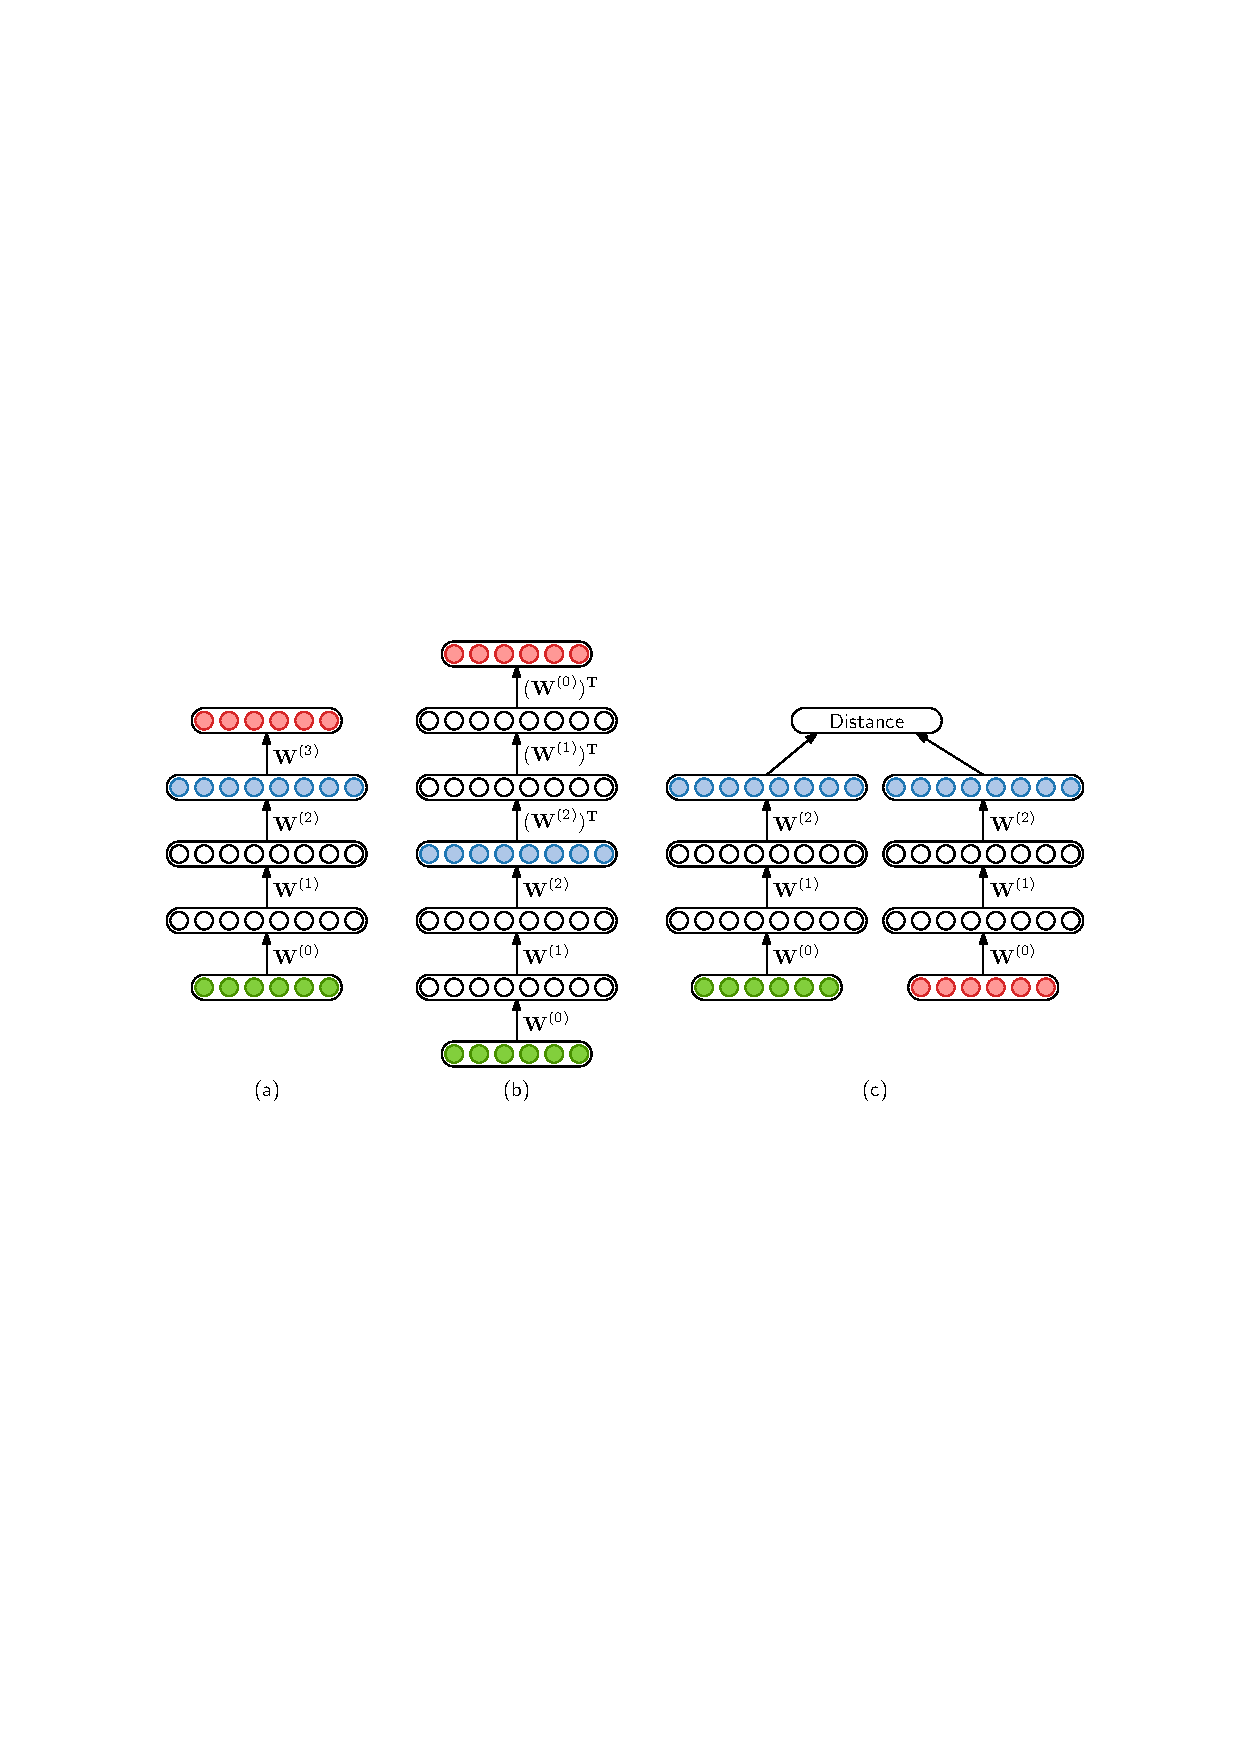
\includegraphics[width=\linewidth]{cae_siamese}
            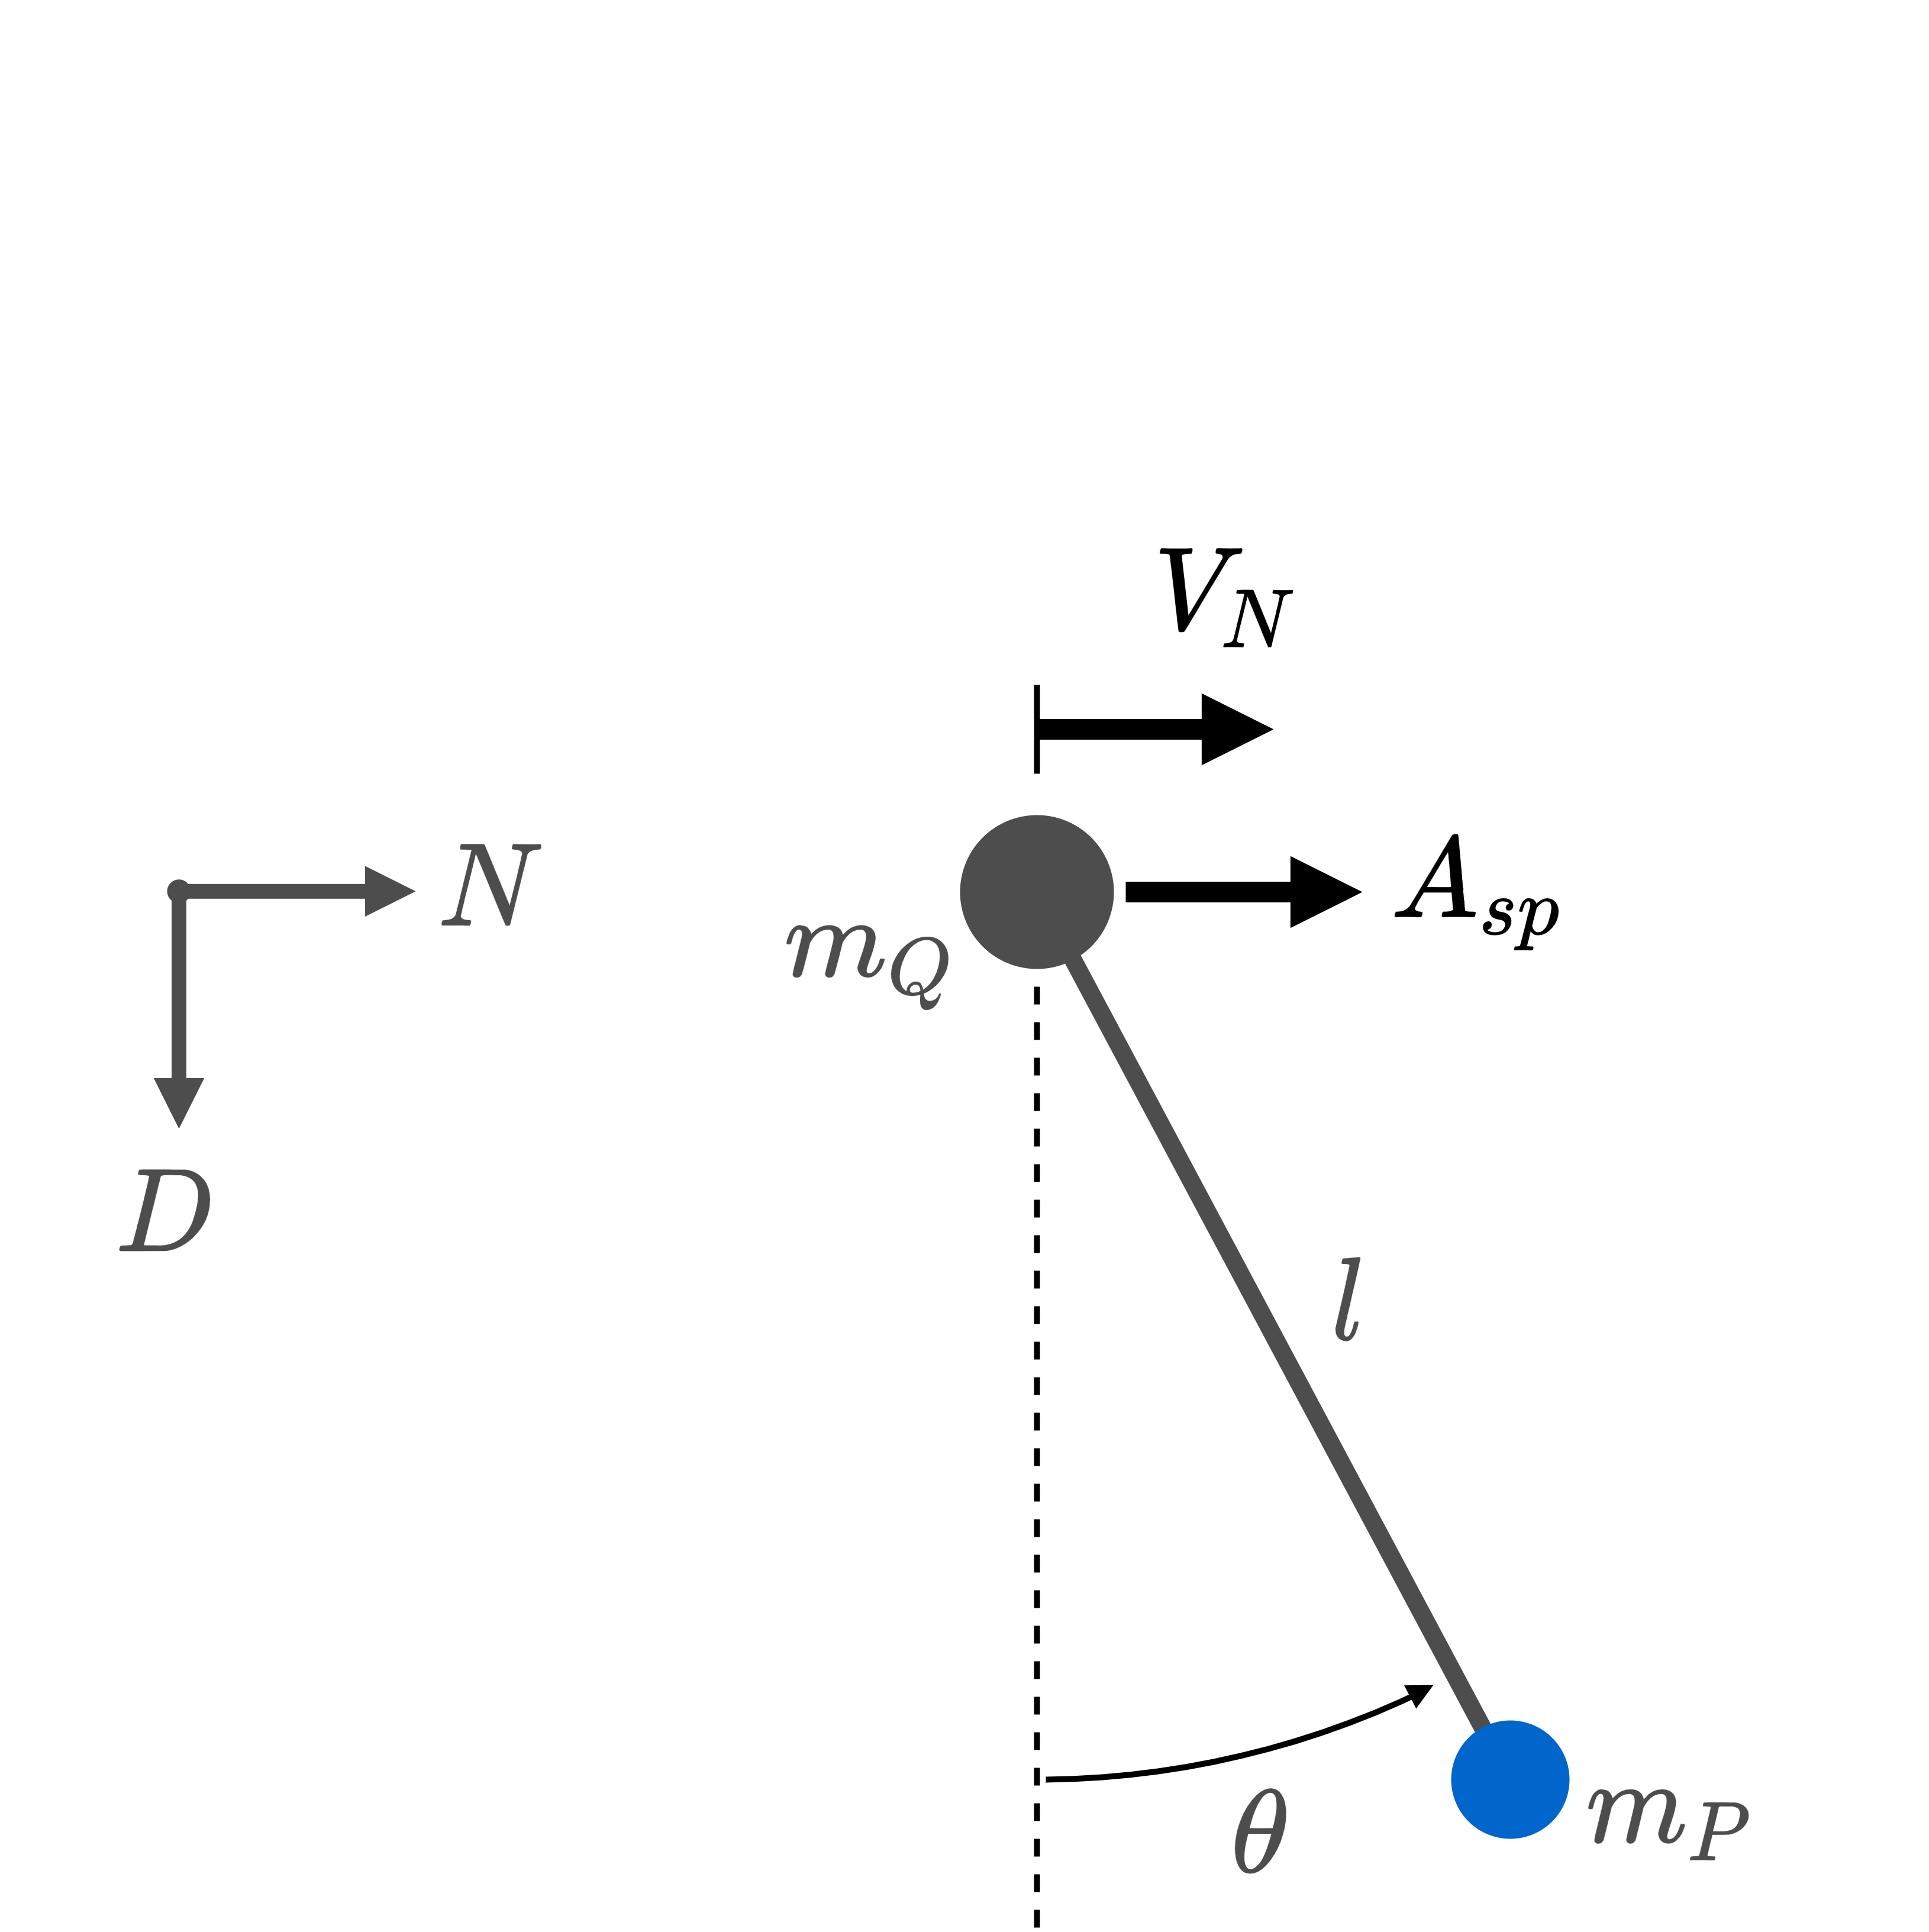
\includegraphics[width=0.5\linewidth]{floating_pend.png}            
            \caption{Floating pendulum model considered for system identification for a North velocity controller}
            \label{fig:floating_pend}
        \end{figure}
    
        \paragraph{Derived model}
        Figure \ref{fig:floating_pend} shows the plant considered for system identification.
        In Chapter~\ref{chap:modelling} the differential equations that describe the motion of this system are derived with Lagrangian mechanics.
        From these equations it is clear that the considered plant is defined by the state vector,
        \begin{equation}
            \bm{x} = \begin{bmatrix}
                V_N & \dot{\theta}
            \end{bmatrix}^T,
        \end{equation}
        and the input vector,
        \begin{equation}
            \bm{u} = \begin{bmatrix}
                A_{N,sp}
            \end{bmatrix},
        \end{equation}
    
        % From this derivation it is clear that the angular velocity of the payload, $\dot{\theta}$, is required to described the system dynamics.
        % However, $\dot{\theta}$ is not measured directly on the considered practical quadrotor setup.
        % Instead, the payload angle, $\theta$, is measured by a potentiometer attached to a ADC on Honeybee as described in Chapter \ref{chap:system_overview}.
        % As expected, this measurement is extremely noisy.
        % \murray{Maybe insert figure to show noise}
        % % Figure \ref{} shows the angle measurement during a practical experiment of the payload while Honeybee is held stationary
        % Numerical differentiation is applied to the noisy $\theta$ signal which results in a very inaccurate estimation of $\dot{\theta}$.
        % Therefore it is desirable to rather use $\theta$ in the system identification process. 

\section{Parameter estimation}
    \subsection{Predetermined linear model}
        The motivation for paramater estimation is to determine unknown parameter values required by the predetermined model.
        This model was derived a prioiri in Section~\ref{sec:linear_model}.
        
    \subsection{Payload mass estimation}
        RLS

    \subsection{Cable length estimation}
        The cable length is estimated from the measurement of natural frequency of the swinging payload.
        As described by
        \cite{bisgaard},
        the natural frequency is given by:
        \begin{equation} \label{eq:nat_freq}
            \omega_n = \sqrt{ \frac{g}{l} \cdot \frac{m_q + m_p}{m_q}}
        \end{equation}
        The natural frequency is measured by performing a FFT on the payload swing angle response after a position step by the quadrotor.
        The dominant frequency identified by the FFT during free swing is the natural frequency of the payload.
        
        \ref{fig:pos_step_angle}
        shows the payload swing angle after the system is stimulated by a position step setpoint.
        As shown in 
        \ref{fig:pos_step_angle}
        the first few seconds of the step response are not used in the FFT.
        This is to minimise the effect of the quadrotor controllers on the swing angle frequency 
        by excluding the transient response in the FFT.

        \ref{fig:fft} 
        shows the resulting amplitude spectrum of the payload swing angle response.
        The dominant frequency is clearly identified as ??.
        Since $m_q$ and $g$ is known, and $m_p$ and $\omega_n$ has been estimated, $l$ can now be determined from
        \ref{eq:nat_freq}.
        In this case the estimated length is ??, compared to the actual length of ??.
        
        Frequency resolution ??
        error for different lengths??
  
\section{Dynamic Mode Decomposition with control}
\label{sec:dmdc}
    
    \paragraph{Intro}        
    DMD is a linear regression technique that can be used to approximate a non-linear dynamical system \cite{Tu2014}.
    It uses temporal measurements of system outputs to reconstruct system dynamics without prior modelling assumptions.
    DMDc is an adaptation of DMD that also accounts for control inputs \cite{Proctor2016c}.
    This section provides an overview of the specific implementation of DMDc used in this paper.        
    Note that this implementation is a slight adaptation of DMDc, and includes time-delay-embedding of multiple observables. 
    \cite{Korda2018b} and \cite{Arbabi2018} use time-delay-embedding in their DMD adaptions in similar ways.

    \paragraph{State space model}
    DMD produces a linear, discrete state-space model of the system dynamics.
    Discrete measurements, $\bm{x}_k$, of the continuous time observable, $\bm{x}(t)$, are used, 
    where $\bm{x}_k = \bm{x}(k T_s)$, and $T_s$ is the sampling time of the model.    
    Delay-coordinates (i.e. $\bm{x}_{k-1}, \bm{x}_{k-2}$, etc.) are also included in the state-space model to
    account for input delay and state delay in the system.
    Input delay refers to the time delay involved with transporting a control signal to a system, 
    whereas state delay refers to time-separated interactions between system variables \cite{Chen1999}.
    Hence, we define an state delay vector as:
    \begin{equation}
        \bm{d}_{k} = 
        \begin{bmatrix}
            \bm{x}_{k-1} & \bm{x}_{k-2} & \cdots & \bm{x}_{k-q}
        \end{bmatrix}^T ,
    \end{equation}
    $\bm{d}_k \in \R^{(n_x)(q)}$ and where $q$ is the number of delay-coordinates used in the model.
    
    \paragraph{}
    The discrete state-space model is therefore defined as:
    \begin{equation} \label{eq:dmd_state_space}
        \bm{x}_{k+1} = \bm{A} \bm{x}_k + \bm{A}_d \bm{d}_k + \bm{B} \bm{u}_k ,
    \end{equation}
    \( \bm{A} \in \R^{n_x \times n_x} \) is the system matrix, 
    \( \bm{A}_1 \in \R^{(q \cdot n_x) \times (q \cdot n_x)} \) is the state delay system matrix and 
    \( \bm{B} \in \R^{n_x \times n_u} \) is the input matrix.
    
    \paragraph{Training data}
    The training data consists of full-state measurements, $\bm{x}_k$, and corresponding inputs, $\bm{u}_k$, 
    taken at regular intervals of $\Delta t = T_s$, during a simulated flight with Cascaded PID control.
    In a practical flight, these time-series measurements need to be saved in memory because it is usd as a single batch by DMD.
    Note that DMD can be applied in a recursive manner as described in \cite{Noack2016}, 
    However this implementation is not considered because memory size will not be a limitation since a companion computer will be used.
    
    \paragraph{Data matrices}
    The training data is collected into the following matrices:
    \begin{align} \label{eq:dmd_matrices}
        \bm{X^\prime} = & \phantom{.} \left [
            \begin{array}{*{5}{@{}M{\mycolwd}@{}}}
                    \bm{x}_{q+2} & \bm{x}_{q+3} & \bm{x}_{q+4} & \cdots & \bm{x}_{w+q+1}
            \end{array}
        \right ] , \nonumber \\
        %
        \bm{X} \phantom{''} = & \phantom{.} \left [
            \begin{array}{*{5}{@{}M{\mycolwd}@{}}}
                \bm{x}_{q+1} & \bm{x}_{q+2} & \bm{x}_{q+3} & \cdots & \bm{x}_{w+q}                      
            \end{array}
        \right ] , \nonumber \\
        % 
        \bm{X}_d \phantom{'} = & \phantom{'} \left [
            \begin{array}{*{5}{@{}M{\mycolwd}@{}}}
                \bm{x}_{q} & \bm{x}_{q+1} & \bm{x}_{q+2} & \cdots & \bm{x}_{w+q-1} \\
                \vdots   & \vdots   & \vdots   & \ddots & \vdots \\
                \bm{x}_2 & \bm{x}_3 & \bm{x}_4 & \cdots & \bm{x}_{w+1} \\
                \bm{x}_1 & \bm{x}_2 & \bm{x}_3 & \cdots & \bm{x}_{w} \\                       
            \end{array}
        \right ] , \nonumber \\
        % 
        \bm{\Upsilon} \phantom{'} = & \phantom{.} \left [
            \begin{array}{*{5}{@{}M{\mycolwd}@{}}}
                    \bm{u}_{q} & \bm{u}_{q+1} & \bm{u}_{q+2} & \cdots & \bm{u}_{w+q-1}
            \end{array}
        \right ] ,
    \end{align}

    where $w$ is the number of columns in the matrices, 
    $\bm{X^\prime}$ is the matrix $\bm{X}$ shifted forward by one time-step, 
    $\bm{X}_d$ is the matrix with delay states, 
    and $\bm{\Upsilon}$ is the matrix of inputs.
    Equation (\ref{eq:dmd_state_space}) can be combined with the matrices in Equation (\ref{eq:dmd_matrices}) to produce:
    \begin{equation}
        \bm{X^\prime} = \bm{A} \bm{X} + \bm{A}_d \bm{X}_d + \bm{B} \bm{\Upsilon} .
    \end{equation}
    Note that the primary objective of DMDc is to determine the best fit model matrices, $\bm{A}$, $\bm{A}_d$ and $\bm{B}$, 
    given the data in $\bm{X^\prime}$, $\bm{X}$, $\bm{X}_d$, and $\bm{\Upsilon}$ \cite{Proctor2016c}.
    In order to group the unknowns into a single matrix, (\ref{eq:dmd_state_space}) is manipulated into the form,
    \begin{equation} \label{eq:G_Omega}
        \bm{X^\prime} =   
        \begin{bmatrix} 
            \bm{A} & \bm{A}_d & \bm{B} 
        \end{bmatrix}
        \begin{bmatrix} 
            \bm{X} \\ \bm{X}_d \\ \bm{\Upsilon} 
        \end{bmatrix} 
        = \bm{G \Omega} ,
    \end{equation} 
    where $\bm{\Omega}$ contains the state and control data, and $\bm{G}$ represents the system and input matrices.
    
    \paragraph{SVD}
    A SVD is performed on $\bm{\Omega}$ resulting in:
    \(
        \bm{\Omega} = \bm{U} \bm{\Sigma} \bm{V}^T
    \).
    Often, only the first $p$ columns of $\bm{U}$ and $\bm{V}$ are required for a good approximation of the dynamics \cite{Brunton2017a}.
    Talk about Reduced Order Modelling??
    POD modes??
    In many cases, the truncated form results in better models than the exact form when noisy measurements are used.
    This is because the effect of measurement noise is mostly captured by the truncated columns of $\bm{U}$ and $\bm{V}$.
    By truncating these columns, the influence of noise in the regression problem is reduced. \murray{explain this better}
    hence the SVD is used in the truncated form: 
    \begin{equation} \label{eq:tilde_svd}
        \bm{\Omega} \approx \Tilde{\bm{U}} \Tilde{\bm{\Sigma}} \Tilde{\bm{V}}^T ,
    \end{equation}
    where $\phantom{.} \Tilde{ } \phantom{.}$ represents rank-$p$ truncation.
    \murray{maybe insert colour pictures showing matrices}        

    \paragraph{}
    By combining (\ref{eq:tilde_svd}) with the over-constrained equality in (\ref{eq:G_Omega}), 
    the least-squared solution, $\bm{G}$, can be found with:
    \begin{equation}
        \bm{G} \approx \bm{X^\prime} \Tilde{\bm{V}} \Tilde{\bm{\Sigma}}^{-1} \Tilde{\bm{U}} .
    \end{equation}
    By reversing \ref{eq:G_Omega}, $\bm{G}$ can now be separated into:
    \(
        \bm{G} = \begin{bmatrix} \bm{A} & \bm{A}_d & \bm{B} \end{bmatrix}.
    \)
    according to the required dimensions of each matrix.
    Thereby, the state-space model approximated by DMDc is complete.
    
\section{Hankel Alternative View Of Koopman} 
\label{sec:havok}
    
    \murray{q = number of delays, from here up}
    
    \paragraph{}
    HAVOK is a data-driven, regression technique that provides a connection between DMD and Koopman operator theory \cite{Brunton2017a, Champion2019}. 
    We have adapted the standard HAVOK algorithm slightly to account for the effect of control and to extract a discrete, linear model that approximates the behaviour of a controlled dynamical system.
    In this section, a brief overview is provided for this implementation and expansion of \mbox{HAVOK}.
    % 
    \paragraph{}
    The extracted discrete state-space model is defined as:
    \begin{equation} \label{eq:havoc_state_space}
        \bm{a}_{k+1} = \Tilde{\bm{A}} \bm{a}_k + \Tilde{\bm{B}} \bm{u}_k ,
    \end{equation}
    where $\bm{a}_k$ is the state vector previously defined in Section \ref{sec:dmdc}, 
    \( \Tilde{\bm{A}} \in \R^{(q \cdot n_x) \times (q \cdot n_x)} \) is the system matrix, 
    and \( \Tilde{\bm{B}} \in \R^{(q \cdot n_x) \times n_u} \) is the input matrix. 
    Here, $\Tilde{\phantom{a}}$ is used to differentiate these matrices from $\bm{A}$ and $\bm{B}$ used in DMDc.
    % 
    \paragraph{}
    The original HAVOK algorithm, developed by \cite{Brunton2017}, constructs a Hankel matrix from output variables only. 
    In order to incorporate the effect of control, an extended Hankel matrix, $\bm{\Pi}$, is created by appending a matrix of inputs to a Hankel matrix of measurements:
    \begin{equation} \label{eq:pi_hankel}
        \bm{\Pi} = \phantom{.} \left [
            \begin{array}{*{5}{@{}M{\mycolwd}@{}}}
                    \bm{a}_{q} & \bm{a}_{q+1} & \bm{a}_{q+2} & \cdots & \bm{a}_{w+q-1} \\
                    \bm{u}_{q} & \bm{u}_{q+1} & \bm{u}_{q+2} & \cdots & \bm{u}_{w+q-1}
            \end{array}
        \right ] ,
    \end{equation}
    where $w$ is the number of columns in $\bm{\Pi}$.
    A truncated SVD of this Hankel matrix results in following approximation:
    \begin{equation} \label{eq:havok_svd_tilde}
        \bm{\Pi} \approx \Tilde{\bm{U}} \Tilde{\bm{\Sigma}} \Tilde{\bm{V}}^T ,
    \end{equation}
    where $\Tilde{\phantom{a}}$ represents rank-$p$ truncation.
    It is important to note that the model extracted by HAVOK depends on the choice of hyperparameters, $p$ and $q$.
    The number of samples in the training data, $N_{train} = w + q -1$, also influences the accuracy of the model.
    % 
    \paragraph{}
    The columns of $\Tilde{\bm{V}}$ are the most significant principal components of the system dynamics \cite{Kamb2020}.
    This matrix, $\Tilde{\bm{V}}$, can be considered to contain a time-series of the pseudo-state, $\bm{v}$, such that
    \(
        \Tilde{\bm{V}}^T = \begin{bmatrix} 
            \bm{v}_q & \bm{v}_{q+1} & \cdots & \bm{v}_w 
        \end{bmatrix} ,
    \)
    characterises the evolution of the actual dynamics in an eigen-time-delay coordinate system \cite{Brunton2017}.
    % 
    Consider the following discrete, state-space formulation:
    \begin{equation} \label{eq:v_ss}
        \bm{v}_{k+1} = \bm{\Lambda} \bm{v}_k .
    \end{equation}
    Recall that DMDc finds a best fit linear operator that directly maps $\bm{a}_{k}$ to $\bm{a}_{k+1}$.
    Similarly, HAVOK determines the best fit linear operator $\bm{\Lambda}$ that maps the pseudo-state $\bm{v}_k$ to $\bm{v}_{k+1}$.
    So, in order to setup an over-determined equality for (\ref{eq:v_ss}), $\Tilde{\bm{V}}^T$ is divided into two matrices:
    \begin{align} \label{eq:v1v2}
        \bm{V}_1 &= \left [
            \begin{array}{*{5}{@{}M{\mycolwd}@{}}} 
                \bm{v}_{q \phantom{-1}}     & \bm{v}_{q+1} & ... & \bm{v}_{w-1} \\
            \end{array} 
        \right ] , \nonumber \\ 
        \bm{V}_2 &= \left [
            \begin{array}{*{5}{@{}M{\mycolwd}@{}}} 
                \bm{v}_{q+1}     & \bm{v}_{q+2} & ... & \bm{v}_{w \phantom{-1}} \\
            \end{array} 
        \right ] ,
    \end{align} 
    where $\bm{V}_2$ is $\bm{V}_1$ advanced a single step forward in time.
    The matrices from Equation (\ref{eq:v1v2}) are now combined with Equation (\ref{eq:v_ss}) and the best fit $\bm{\Lambda}$ is determined with the Moore-Penrose pseudoinverse:
    \begin{equation} \label{eq:v_dmd}
        \bm{V}_2 = \bm{\Lambda} \bm{V}_1 \phantom{---} \Rightarrow \phantom{---} \bm{\Lambda} \approx \bm{V}_1 \bm{V}_1^{\dagger}
    \end{equation}
    % 
    It can be shown from Equation (\ref{eq:havok_svd_tilde}) that Equation (\ref{eq:v_ss}) is transformed from the eigen-time-delay coordinate system to the original coordinate system as the following:
    \begin{equation} \label{eq:v_ss_a} 
        \begin{bmatrix}
            \bm{a}_{k+1}  \\  \bm{u}_{k+1} 
        \end{bmatrix}
    \phantom{.} = \phantom{.} (\Tilde{\bm{U}} \Tilde{\bm{\Sigma}}) \bm{\Lambda} (\Tilde{\bm{U}}  \Tilde{\bm{\Sigma}})^{\dagger} \phantom{.}
        \begin{bmatrix}
            \bm{a}_{k}  \\  \bm{u}_{k} 
        \end{bmatrix} .
    \end{equation}    
    % 
    This form is used to extract $\Tilde{\bm{A}}$ and $\Tilde{\bm{B}}$ from the matrix,
    \( 
        (\Tilde{\bm{U}} \Tilde{\bm{\Sigma}}) \bm{\Lambda} (\Tilde{\bm{U}}  \Tilde{\bm{\Sigma}})^{\dagger}
    \), in the following way:
    \begin{equation} \label{matrix_decomp}
        \begin{bmatrix}
            \bm{a}_{k+1}  \\  \bm{u}_{k+1} 
        \end{bmatrix}
        \phantom{.} = \phantom{.} 
        \begin{bmatrix}
            \Tilde{\bm{A}} \phantom{.....} \Tilde{\bm{B}} \\
            \textit{(discarded)}
        \end{bmatrix}
        \phantom{.}
        \begin{bmatrix}
            \bm{a}_{k}  \\  \bm{u}_{k} 
        \end{bmatrix}.
    \end{equation}    
    % 
    % This decomposition is illustrated in Fig.~\ref{fig:lambda_decomp}, where blocks represent different groups of entries in the matrix.
    % \begin{figure}[h]
    %     \includegraphics[scale = 0.45]{Lambda_decomp.png}
    %     \centering
    %     \caption{Illustration of the extraction of $\Tilde{\bm{A}}$ and $\Tilde{\bm{B}}$ from (\ref{eq:v_ss_a})}
    %     \label{fig:lambda_decomp}
    % \end{figure}
    % 
    Note that the matrix entries in (\ref{matrix_decomp}) that map $\bm{u}_k$ to $\bm{u}_{k+1}$ are meaningless for our purposes and are discarded.
    Similarly to DMDc, some matrix entries in $\Tilde{\bm{A}}$ and $\Tilde{\bm{B}}$ are known a priori due to the relative positions of delay coordinates. These are forced to 1 or 0 to improve the prediction performance of the model.
    
    \murray{merge these paragraphs}
    Since the state vector, $\bm{a}$, includes delay-coordinates, some matrix entries are known a priori and are independent of the dynamics. 
    For example, the values of $\bm{x}_{k}$ should be mapped from their position in $\bm{a}_k$ to specific indices in $\bm{a}_{k+1}$. 
    Due to the least-squares fitting and coordinate transformation, DMDc will not produce these exact values in $\bm{A}$ and $\bm{B}$. 
    By forcing each of these matrix entries to 1 or 0, the state-prediction performance of the model is improved.




\section{Implementation and results}
    \subsection{Methodology}
        \paragraph{Simulation environment}

        \paragraph{Method overview}
        \murray{Maybe convert this to a flow diagram}

        \begin{enumerate}
            \item Takeoff and hover
            \item Command a series of velocity step inputs with random step sizes and time intervals
            \item Measure and save input and output data
            \item Apply algorithm to data and generate model
        \end{enumerate}

        \paragraph{}

        \paragraph{Steps and intervals}
        For the training period, different velocity step inputs are commanded with varying time intervals between step commands.
        A algorithm schedules these velocity step commands, by assigning random step values and time-intervals within a specified range.
        The velocity range is determined in simulation by iteratively increasing the maximum velocity step 
        to a safe value where the quadrotor and payload system remain in stable flight.
        The maximum time-interval is set to a value that allows the payload swing to reach a steady-state condition.
        This ensures that the identified model includes transient and steady-state dynamics.

        \paragraph{Why velocity steps?}
        Velocity step commands are used in the training period because this 
        Frequency decomposition stimulates the system for a large range of frequencies.

        \paragraph{Testing data}
        Cross-validate

        \paragraph{Error metric}
        Each state error signal is scaled by the reciprocal of the maximum value of that state variable in the training data.
        % This is to provide a better representative error when taking the mean of state variable errors.
        This is to ensure that a scale difference in the variable types create a bias in the error metric.
        For example, the quadrotor velocity reaches values of \SI{3}{\metre/\second} but the payload swing angle has a maximum of only \SI[]{0.526}{\radian}.
        The velocity prediction error is therefore inherently larger than the payload angle prediction error
        and will bias the error metric towards favouring models with good velocity predictions.
        The proposed scaled error metric ensures that the MAE of each state variable can be compared to each other.
        It also provides an error metric that is better and unbiased representative of the model prediction performance across all state variables. 

        Add Information Criteria ??
        AIC Brunton Kutz??

    \subsection{Hyperparameters}
        As discussed in Section~\ref{sec:dmdc} and \ref{sec:havok} 
        DMDc and HAVOK are dependent on two hyperparameters: the number of delay-coordinates, $q$, and the SVD truncation rank, $p$.

        Parsimony
        Pareto front
        cite Data-Driven book

        The more terms better chance to overfit, lower generalisation
        \begin{figure}[htb]
    \centering
    \begin{tikzpicture}
        \begin{axis}[            
            xlabel = {Number of delay-coordinates, $q$},
            ylabel = $\overline{NMAE}$ \phantom{~},
            % x unit = \si{\second},
            y unit = \%,
            xmin = 2,     xmax = 40,
            ymin = 3.2,  ymax = 6.5,
            grid = major,
            legend cell align = left,
            legend pos = north east,
            grid style = dashed,
            legend style = {font = \scriptsize},
            label style = {font = \scriptsize},
            tick label style = {font = \scriptsize},
            width = 0.95\columnwidth,
            height = 0.5\columnwidth,
            % initialize Dark2
            cycle list/Dark2,
            % combine it with 'mark list*':
            cycle multiindex* list = {
                Dark2\nextlist
            }
        ]

        \addplot+[mark = none, style = solid, ultra thick] 
        table[x = q, y expr = {\thisrow{NMAE_mean}*100}, col sep = comma] 
        {system_id/csv/NMAE_vs_q_SITL_x_vel_noise_longer_times_q.csv_dmd_angle_Ttrain_60.csv};
        \addlegendentry{DMD}
        
        \addplot+[mark = none, style = solid, ultra thick] 
        table[x = q, y expr = {\thisrow{NMAE_mean}*100}, col sep = comma] 
        {system_id/csv/NMAE_vs_q_SITL_x_vel_noise_longer_times_q.csv_havok_angle_Ttrain_60.csv};
        \addlegendentry{HAVOK}

        \end{axis}
    \end{tikzpicture} 
    
    \caption{\gls{DMD} and \gls{HAVOK} predictions error for different lengths of noisy training data
    ($m_p =$~\SI{0.2}{\kilo\gram}, $l =$~\SI{0.5}{\meter}, $T_s =$~\SI{0.03}{\second}, $T_{train} =$~\SI{60}{\second}.)}
    \label{fig:NMAE_vs_q}
\end{figure}


        % \begin{figure}[htb]
    \centering
    \begin{tikzpicture}
        \begin{semilogyaxis}[            
            xlabel = Index of mode,
            ylabel = Singular value,
            % x unit = \si{\second},
            % y unit = \si{\second},
            xmin = 0,     xmax = 60,
            ymin = 1e-2,  ymax = 1e3,
            grid = major,
            legend cell align = left,
            legend pos = north east,
            grid style = dashed,
            legend style = {font = \scriptsize},
            label style = {font = \scriptsize},
            tick label style = {font = \scriptsize},
            width = 0.95\columnwidth,
            height = 0.5\columnwidth,
            % initialize Dark2
            cycle list/Dark2,
            % combine it with 'mark list*':
            cycle multiindex* list = {
                Dark2\nextlist
            }
        ]

        \addplot+[only marks, mark = square, ultra thick] 
        table[x = index, y = S, col sep = comma] 
        {system_id/csv/Singular_values_SITL_x_vel_noise_longer_times_q.csv_havok_angle_Ttrain_60_q29_p13.csv};
        \addlegendentry{Significant modes}

        \addplot+[only marks, mark = square, ultra thick] 
        table[x = index, y = S, col sep = comma] 
        {system_id/csv/Singular_values_SITL_x_vel_noise_longer_times_q.csv_havok_angle_Ttrain_60_q29_p13_trunc.csv};
        \addlegendentry{Truncated modes}

        \end{semilogyaxis}
    \end{tikzpicture} 
    
    \caption{Significant and truncated singular values of a \gls{HAVOKc} model produced from noisy data
    ($m_p =$~\SI{0.2}{\kilo\gram}, $l =$~\SI{0.5}{\meter}, $T_s =$~\SI{0.03}{\second}, $T_{train} =$~\SI{60}{\second}.).}
    \label{fig:singular_values}
\end{figure}


        Fixed size of data
        Fixed sample time
        Fixed pendulum params
        Talk about the "front"
        Also about singular values
        For each of the experiments shown in this chapter, a hyperparameters selected tuned to produced

    \subsection{Sample time}
        best hyperparameters.
        best N_train.
        \begin{figure}[htb]
    \centering
    \begin{tikzpicture}
        \begin{axis}[            
            xlabel = Ts,
            ylabel = $\overline{NMAE}$ \phantom{~},
            % x unit = \si{\second},
            y unit = \%,
            xmin = 0,     xmax = 0.07,
            ymin = 8.5,  ymax = 12.5,
            grid = major,
            legend cell align = left,
            legend pos = north east,
            grid style = dashed,
            legend style = {font = \scriptsize},
            label style = {font = \scriptsize},
            tick label style = {font = \scriptsize},
            width = 0.95\columnwidth,
            height = 0.5\columnwidth,
            % initialize Dark2
            cycle list/Dark2,
            % combine it with 'mark list*':
            cycle multiindex* list = {
                Dark2\nextlist
            }
        ]

        \addplot+[mark = none, style = solid, ultra thick] 
        table[x = Ts, y expr = {\thisrow{NMAE_mean}*100}, col sep = comma] 
        {system_id/csv/NMAE_vs_Ts_SITL_x_vel_noise_longer_times_Ts.csv_dmd_angle.csv};
        \addlegendentry{DMD}
        
        \addplot+[mark = none, style = solid, ultra thick] 
        table[x = Ts, y expr = {\thisrow{NMAE_mean}*100}, col sep = comma] 
        {system_id/csv/NMAE_vs_Ts_SITL_x_vel_noise_longer_times_Ts.csv_havok_angle.csv};
        \addlegendentry{HAVOK}

        \end{axis}
    \end{tikzpicture} 
    
    \caption{DMD and HAVOK predictions error for different sample times of noisy training data
    ($m =$~\SI{0.2}{\kilo\gram}, $l =$~\SI{0.5}{\meter}, $T_{train} =$~\SI{60}{\second}.)}
    % \label{fig:havok_vs_dmd_noise}
\end{figure}

        Fixed size of data.
        Fixed pendulum params.

    \subsection{Choice of payload variable in the state vector}
        As discussed in Section~\ref{sec:plant_considered}, 
        the equations of motion of a floating pendulum in continuous-time are dependent on $\dot{\theta}$ and $V_N$, 
        but are not dependent on $\theta$.
        Therefore it is expected that 
        $
        \bm{x} = \begin{bmatrix}
            V_N & \dot{\theta}
        \end{bmatrix}^T
        $
        is used as the state vector for system identification.
        However, if $\dot{\theta}$ is not included in the state vector of a discrete model, 
        it can still be represented with numerical differentiation like the backward Euler form,
        \begin{equation}
            \dot{\theta}_k = (\frac{1}{T_s}) \cdot \theta_k - (\frac{1}{T_s}) \cdot \theta_{k-1} .
        \end{equation}
        Therefore the original state vector can also be replaced by,
        $
            \bm{x} = \begin{bmatrix}
                V_N & \theta
            \end{bmatrix}^T
        $
        in system identification.

        \paragraph{}
        Based on the floating pendulum equations, it is expected that a model derived with $\dot{\theta}$ data 
        will better approximate the actual dynamics than one using $\theta$.
        This is because $\dot{\theta}$ contains more direct information about the dynamics compared to $\theta$.
        A model using $\theta$ needs to "learn" numerical differentiation and the effect of $\dot{\theta}$ on the other variables.
        A model using $\dot{\theta}$ only needs to consider its relationship with other variables.

        \begin{figure}[h]
    \centering
    \begin{tikzpicture}
        \begin{axis}[            
            xlabel = Length of training data,
            ylabel = MAE,
            x unit = \si{\second},
            % y unit = \si{\second},
            xmin = 0,     xmax = 120,
            ymin = 0.0005, ymax = 0.08,
            grid = major,
            legend cell align = left,
            legend pos = north east,
            grid style = dashed,
            legend style = {font = \scriptsize},
            label style = {font = \scriptsize},
            tick label style = {font = \scriptsize},
            width = 0.95\columnwidth,
            height = 0.5\columnwidth,
            % initialize Dark2
            cycle list/Dark2,
            % combine it with 'mark list*':
            cycle multiindex* list = {
                Dark2\nextlist
            }
        ]
         
        \addplot+[mark = none, style = solid, ultra thick] 
        table[x = T_train, y = MAE_mean, col sep = comma] 
        {system_id/csv/MAE_vs_Ntrain_Simulink_single_pend_mp0.2_l0.5_PID_vel_steps_tune_scale_0.7longer_times.mat_dmd_angle.csv};
        \addlegendentry{DMD with $\theta$}

        \addplot+[mark = none, style = solid, ultra thick] 
        table[x = T_train, y = MAE_mean, col sep = comma] 
        {system_id/csv/MAE_vs_Ntrain_Simulink_single_pend_mp0.2_l0.5_PID_vel_steps_tune_scale_0.7longer_times.mat_havok_angle.csv};
        \addlegendentry{HAVOK with $\theta$}
        
        \addplot+[mark = none, style = dashed, ultra thick] 
        table[x = T_train, y = MAE_mean, col sep = comma] 
        {system_id/csv/MAE_vs_Ntrain_Simulink_single_pend_mp0.2_l0.5_PID_vel_steps_tune_scale_0.7longer_times.mat_dmd_angular_rate.csv};
        \addlegendentry{DMD with $\dot{\theta}$}

        \addplot+[mark = none, style = dashed, ultra thick] 
        table[x = T_train, y = MAE_mean, col sep = comma] 
        {system_id/csv/MAE_vs_Ntrain_Simulink_single_pend_mp0.2_l0.5_PID_vel_steps_tune_scale_0.7longer_times.mat_havok_angular_rate.csv};
        \addlegendentry{HAVOK with $\dot{\theta}$}

        \end{axis}
    \end{tikzpicture} 
    
    \caption{Prediction MAE for models using angle or angular rate measurements 
    ($m =$~\SI{0.2}{\kilo\gram}, $l =$~\SI{0.5}{\meter}, $T_s =$~\SI{0.03}{\second}).}
    \label{fig:SITL_MAE_vs_train_angular_rate}
\end{figure}


        \paragraph{}
        % Figure~\ref{} shows the prediction error of techniques using $\dot{\theta}$ or $\theta$ for different amounts of training data.
        For each length of training data, the hyperparameter combination producing the lowest prediction error was determined and used.
        From this plot it is clear that models with $\theta$ produce more accurate predictions than those with $\dot{\theta}$.

    \subsection{Noise}
        \paragraph{}
        Measurement noise is \murray{Find reference for measurement noise definition}
        This is bad for system identification because the output signals no longer represent the actual process
        hides the actual dynamics of the system under  
        The IMU, barometer, magnetometer and GPS sensors on the practical quadrotor are used for state estimation 
        and all experience measurement noise.
        The EKF performs sensor fusion and smooths out most of the measurement noise to provide a state estimate that is less noisy than raw sensor values.
        
        \paragraph{}
        The potentiometer and ADC which measure the payload angle on the quadrotor alos has quite a lot of measurement noise.
        However, this signal is not smoothed by an onboard EKF.
        Figure~\ref{fig:payload_noise} shows the noisy payload angle measurement for a practical pendulum test while the quadrotor is held stationary.
        For models using $\theta$ in the state vector instead of $\dot{\theta}$, 
        this noisy signal can be smoothed with \murray{matlab smoother}.
        Figure~\ref{fig:payload_noise_smoothed} compares the noisy payload angle measurement to the smoothed signal and actual payload angle for a simulated flight.
        The is applied as band-limited white-noise and the noise power was iteratively adjusted to match that of the practical payload measurements.
        
        \paragraph{}
        However, since there is no direct measurement of $\dot{\theta}$, 
        numerical differentiation is performed on the noisy $\theta$ measurement to estimate $\dot{\theta}$. 
        This amplifies the noise and results in inaccurate $\dot{\theta}$ signal.
        Total variation differentiation is implemented to estimate $\dot{\theta}$ from the noisy measurements more accurately. \cite{}
        Figure~\ref{fig:payload_noise_diff} shows
        
        % \input{system_id/plots/payload_noise_diff.tex} // With TVDiff

        Noise also affects model prediction accuracy and the length of training data required for adequate predictions. 
        
        \begin{figure}[htb]
    \centering
    \begin{tikzpicture}
        \begin{axis}[            
            xlabel = Length of training data,
            ylabel = $\overline{NMAE}$ \phantom{~},
            x unit = \si{\second},
            y unit = \%,
            xmin = 5,     xmax = 120,
            ymin = 3.2,  ymax = 5.7,
            grid = major,
            legend cell align = left,
            legend pos = north east,
            grid style = dashed,
            legend style = {font = \scriptsize},
            label style = {font = \scriptsize},
            tick label style = {font = \scriptsize},
            width = 0.95\columnwidth,
            height = 0.5\columnwidth,
            % initialize Dark2
            cycle list/Dark2,
            % combine it with 'mark list*':
            cycle multiindex* list = {
                Dark2\nextlist
            }
        ]

        \addplot+[mark = none, style = solid, ultra thick] 
        table[x = T_train, y expr = {\thisrow{NMAE_mean}*100}, col sep = comma] 
        {system_id/csv/NMAE_vs_Ntrain_SITL_x_vel_no_noise_longer_times.csv_havok_angle.csv};
        \addlegendentry{Without noise}

        \addplot+[mark = none, style = solid, ultra thick] 
        table[x = T_train, y expr = {\thisrow{NMAE_mean}*100}, col sep = comma] 
        {system_id/csv/NMAE_vs_Ntrain_SITL_x_vel_noise_longer_times.csv_havok_angle.csv};
        \addlegendentry{With noise}

        \end{axis}
    \end{tikzpicture} 
    
    \caption{\gls{HAVOK} prediction errors for different lengths of training data with and without noise 
    ($m_p =$~\SI{0.2}{\kilo\gram}, $l =$~\SI{0.5}{\meter}, $T_s =$~\SI{0.03}{\second}).}
    \label{fig:noise_vs_no_noise}
\end{figure}


        \begin{figure}[htb]
    \centering
    \begin{tikzpicture}
        \begin{axis}[            
            xlabel = Length of training data,
            ylabel = $\overline{NMAE}$ \phantom{~},
            x unit = \si{\second},
            y unit = \%,
            xmin = 5,     xmax = 120,
            ymin = 3.2,  ymax = 5.7,
            grid = major,
            legend cell align = left,
            legend pos = north east,
            grid style = dashed,
            legend style = {font = \scriptsize},
            label style = {font = \scriptsize},
            tick label style = {font = \scriptsize},
            width = 0.95\columnwidth,
            height = 0.5\columnwidth,
            % initialize Dark2
            cycle list/Dark2,
            % combine it with 'mark list*':
            cycle multiindex* list = {
                Dark2\nextlist
            }
        ]

        \addplot+[mark = none, style = solid, ultra thick] 
        table[x = T_train, y expr = {\thisrow{NMAE_mean}*100}, col sep = comma] 
        {system_id/csv/NMAE_vs_Ntrain_SITL_x_vel_noise_longer_times.csv_dmd_angle.csv};
        \addlegendentry{DMD}

        \addplot+[mark = none, style = solid, ultra thick] 
        table[x = T_train, y expr = {\thisrow{NMAE_mean}*100}, col sep = comma] 
        {system_id/csv/NMAE_vs_Ntrain_SITL_x_vel_noise_longer_times.csv_havok_angle.csv};
        \addlegendentry{HAVOK}

        \end{axis}
    \end{tikzpicture} 
    
    \caption{\gls{DMD} and \gls{HAVOK} prediction errors for different lengths of noisy training data
    ($m_p =$~\SI{0.2}{\kilo\gram}, $l =$~\SI{0.5}{\meter}, $T_s =$~\SI{0.03}{\second}).}
    \label{fig:havok_vs_dmd_noise}
\end{figure}


        HAVOK performs better than DMD.
        This slight difference in prediciton performance has a negligible effect on control.
        

        Input data needs to be adjusted.

        % \input{plot of SITL acc_sp}
    

    \subsection{Size of training data}
        The length of training data used for system identification affects the quality of the model produced.
        In Figure~\ref{fig:SITL_MAE_vs_train_angular_rate} it is clear that prediction error decreases as the amount of training data increases.
        As more training data is used in the regression problem, 
        the determined model better approximates the actual dynamics because a large range of the dynamics is "seen" by the algorithm.

        
        % \input{low data prediction}
        \paragraph{}
        Models produced from data lengths as short as \SI{5}{\second} predict the movement of state variables surprisingly well.
        % Figure~\ref{} shows prediction.
        Note how the general shape of the prediction represents the training data, 
        even though it contains a lot more high frequency oscillations.

        \begin{figure}[htb]
    \centering
    \begin{tikzpicture}
        \begin{axis}[            
            xlabel = Length of training data,
            ylabel = NMAE of time derivative of predictions,
            x unit = \si{\second},
            % y unit = \si{\second},
            xmin = 0,     xmax = 120,
            ymin = 0.004,  ymax = 0.016,
            grid = major,
            legend cell align = left,
            legend pos = north east,
            grid style = dashed,
            legend style = {font = \scriptsize},
            label style = {font = \scriptsize},
            tick label style = {font = \scriptsize},
            width = 0.95\columnwidth,
            height = 0.5\columnwidth,
            % initialize Dark2
            cycle list/Dark2,
            % combine it with 'mark list*':
            cycle multiindex* list = {
                Dark2\nextlist
            }
        ]

        \addplot+[mark = none, style = solid, ultra thick] 
        table[x = T_train, y expr = {\thisrow{NMAE_mean}*100}, col sep = comma] 
        {system_id/csv/NMAE_vs_Ntrain_SITL_x_vel_noise_longer_times_MAEdiff.csv_dmd_angle.csv};
        \addlegendentry{DMD}
        
        \addplot+[mark = none, style = solid, ultra thick] 
        table[x = T_train, y expr = {\thisrow{NMAE_mean}*100}, col sep = comma] 
        {system_id/csv/NMAE_vs_Ntrain_SITL_x_vel_noise_longer_times_MAEdiff.csv_havok_angle.csv};
        \addlegendentry{HAVOK}

        \end{axis}
    \end{tikzpicture} 
    
    \caption{DMD and HAVOK error of time derivative of predictions for different lengths of noisy training data
    ($m =$~\SI{0.2}{\kilo\gram}, $l =$~\SI{0.5}{\meter}, $T_s =$~\SI{0.03}{\second}).}
    % \label{fig:havok_vs_dmd_noise}
\end{figure}


        \paragraph{}
        % Figure~\ref{} shows the MAE of prediction state derivative.
        Define MAE diff with equation ??.
        % From Figure~\ref{} it appears that at least \SI{}{} training data is required to produce models that represent the dynamics.

        \paragraph{}
        The models produced from HAVOK appear to produce slightly better prediction errors, however this small difference has a negligible effect on control performance.

        \paragraph{}
        % In Figure~\ref{fig:MAE_vs_train} it can be seen that after approximately \SI{??}{\second} 
        the prediction error does not significantly improve with more training data.
        It practice less training data is desirable because less flight time will be wasted on training a model before the quadrotor can fly with a updated controller.
        Less training data also corresponds to lower memory usage on quadrotor hardware.
        Such a slight improvement in prediction error also has a negligible effect on control performance and is therefore not worth the increased data requirement.
        % Therefore, only \SI{??}{\second} of flight data will be used to train system identification models. 


    \subsection{System parameters}
        Best hyperparameters.
        Fixed size of data.
        Fixed sample time.

    \subsection{Dynamic payload}
        Data-driven vs Parameter estimation

        plot hyperparameterss MAE. Not how much more delays are required

    \subsection{Practical flight data}
    \subsection{HIL}
        \paragraph{Companion computer}
        \paragraph{Software}
        \paragraph{CPU}
        \paragraph{Memory}

